\documentclass[12pt,a4paper,final,oneside,onecolumn,titlepage]{article}
\usepackage{times}
\usepackage{geometry}
\usepackage{fancyhdr}
\usepackage{setspace}
\usepackage{natbib}
\usepackage{amssymb}
\usepackage{graphicx}
\usepackage{sectsty}
\usepackage[table,xcdraw]{xcolor}
\usepackage{polski}
\usepackage[utf8]{inputenc}
\usepackage[T1]{fontenc}
\usepackage[pagewise]{lineno}
\newgeometry{tmargin=2.5cm, bmargin=2.5cm, lmargin=2.5cm, rmargin=2.5cm}
\setlength{\parindent}{3in}
\setlength{\parskip}{0pt}
\linenumbers
\doublespacing
\sectionfont{\centering}
\renewcommand{\bibsection}{\section*{\large{\textbf{\textsc{\centering{Literatura}}}}}}

\begin{document}
\pagestyle{fancy}
\fancyhead{}
\fancyfoot{}
\chead{Nasze otoczenie i funkcje poznawcze}
\rhead{\thepage}
\bibliographystyle{apalike}
\begin{titlepage}
  \thispagestyle{empty}
  \rhead{\thepage}
  \begin{center}
  \vspace*{1cm}
  \Large
  \textbf{\textsc{Nasze otoczenie i funkcje poznawcze:\\ Badanie zależności między entropią informacyjną \textit{(H)} w otoczeniu oraz wykonaniu treningu uważności, a selektywną uwagą wzrokową.\\}}
  \vspace{1.5cm}
  \textit{Laura Plichta, Wiktor Warchałowski, Zofia Załęska\\}
  Wydział Nauk o Zdrowiu, Gdański Uniwersytet Medyczny\\
  \vspace{3cm}
  Praca zaliczeniowa z przedmiotu \\ Metodologia Badań Psychologicznych 2 \\ napisana pod kierunkiem dr. Krzysztofa Basińskiego\\
  \vspace{3cm}
  Gdańsk, 20 Stycznia 2023
  \end{center}
\end{titlepage}
\begin{center}
  \vspace*{0.5cm}
  \large{\textbf{\textsc{Abstrakt}}}
\end{center}
\paragraph{}
Celem niniejszego artykułu jest zbadanie problematyki związanej z wpływem środowiska w jakim się znajdujemy na zdolności poznawcze człowieka. Artykuł ten sprawdza czy istnieje wpływ entropii informacji zaindukowanej przez różnorodność obiektów w otoczeniu i wykonaniem treningu uważności jakim jest kolorowanie mandali na selektywną uwagę wzrokową. Badanie zostało przeprowadzone na 30 osobach, które dobrowolnie zgodziły się na wzięcie udziału w eksperymencie. Indukowana entropia otoczenia została opisana jako różnorodność kulek do basenu dziecięcego w pomieszczeniu, zaś trening uważności jako wykonanie kolorowanki z mandalą. Zmienną niezależną była uwaga wzrokowa, zbadana za pomocą testu Eriksena. Mediany porównywanych grup oraz nieparametryczne testy statystyczne wykazały istnotne różnice w grupach, oraz fakt interakcji zmiennych entropii oraz treningu uważności, jednakże współczynnik d Cohena wskazał siłę efektu, która może uznać efekty za nieistotne w populacji.
\\
\textit{Słowa kluczowe: środowisko, entropia informacji, uwaga wzrokowa, trening uważności}
\newpage
\begin{center}
\section*{\large{\textbf{\textsc{Wstęp}}}}
\end{center}
\paragraph{}
Ze względu na rozwój techniki, kończące się zasoby naturalne, zwiększająca się liczba ludności oraz inne problemy dynamicznie rozwijającego się świata wzrosło zainteresowanie badaniami zależności między człowiekiem, a jego środowiskiem. Dziedziną zajmującą się relacją ludzi i ich zachowań z różnymi modalnościami ich otoczenia oraz jego optymalizacją \citep{banka_psychologia_2018, gifford_environmental_2011}. Dostrzeganie interakcji człowieka ze środowiskiem mogą być czymś ważnym w rozwoju architektury i planowania przestrzennego, aby era antropocenu nie była stworzona destruktywnym wpływem człowieka na naturę, ale okresem w którym działamy na wspólną korzyć \citep{zalasiewicz_new_2010}. Oprócz celu zrównoważnonego rozwoju w celu odpowiedzi na zmiany klimatyczne, badacze zajmują się optymalizacją naszego najbliższego otoczenia. Przykładem takiego działania są badania \citet{lohr_interior_1996} pokazujące zależność struktury miejsca pracy z produktywnością. Jednakże analiz tego typu jest relatywnie mało, ale ich ilość wzrasta w XXI wieku \citep{spano_human_2020}. Inspirując się takim typem eksperymentów, celem niniejszego badania było sprawdzenie, jak modyfikacja środowiska pracy wpłynie na efektywność procesów poznawczych człowieka z naciskiem na selektywną uwagę wzrokową. Aby zuniwersalizować manipulację wyglądem otoczenia, zostało zastosowane pojęcie entropii informacji zgodnie z teorią Shannona. Oznacza to, że fizyczna miara nieuporządkowania i chaosu, jest interpretowana jako suma średnich prawdopodobieństw wystąpienia danego typu informacji i zdarzeń. Jest wyrażana wzorem:
\begin{center}
\begin{math}
H_f=-\displaystyle\sum_{i=1}^{n}p_i\log_2({p_i})
\end{math}
\end{center}
Gdzie $n$ oznacza ilość obiektów, $i$ to dany obiekt, zaś $p$ jest prawdopodobieństwem jego wystąpienia. Wynik powyższego działania podawany jest w bitach \citep{stamps_entropy_2004}. Dodatkowo na potrzeby analizy otoczenia entropia informacji jest liczona jako zróżnicowanie elementów architektonicznych lub dekoracyjnych \citep{stamps_entropy_2004, stamps_entropy_2002}. Ze względu na fakt badania odbioru otoczenia pod względem artystyczno-wizualnym, zdecydowano o dołączeniu kolorowania kolorowanki uważności. Jest to jeden z rodzajów treningu \textit{mindfulness} (z ang. uważność), który polega na pełnej koncentracji na przebiegu kolorowania \citep{zejmo_praktyka_2022}. W ostatnich czasach rośnie również ich popularnosć i rośnie ich rola w życiu codziennym wielu ludzi \citep{dresler_doing_2019}. Stąd dodatkowo ten artykuł sprawdza ich użyteczność co również może pomóc w rozwoju świadomości na temat uwagi i uwarunkowań jej działania. Z tego względu postawionym pytaniem badawczym jest czy zwiększona entropia informacji w kolorach elementów otoczenia oraz wykonanie treningu uważności ma wpływ na selektywną uwagą wzrokową? Przewiduje się, że Zwiększona entropia informacji w kolorach i kształtach elementów otoczenia zmniejsza czas wykonania testu selektywnej uwagi wzrokowej. Dzieje się tak ze względu na fakt, że zwiększona entropia wpływa bezpośrednio na zwiększenie przyjemności i pozytywnego pobudzenia \citep{stamps_entropy_2004, stamps_entropy_2002}, które wpływa na możliwości percepcyjne jednostki, dzięki czemu osoby, którym indukowano przyjemność i pozytywne pobudzenie lepiej radziły sobie z wykonaniem testów percepcyjnych, uwagi wzrokowej oraz ogólnie procesów poznawczych \citep{mcconnell_upbeat_2011, gavazzi_pleasure_2021}. Wykonanie testu uważności również zmniejsza czas wykonania testu selektywnej uwagi wzrokowej ze względu na fakt, że czynność kolorowania mandali pomaga w uspokojeniu się oraz poprawia uważność oraz ogólny stan osoby która koloruje (\textit{mindfulness and wellbeing}) \citep{carsley_effectiveness_2018, campenni_effects_2020}. Wysoki poziom uważności (\textit{mindfulness}) zaś podwyższa poziom uwagi wzrokowej i pomaga w skupieniu się \citep{campillo_effects_2018, sumantry_meditation_2021}. Jednakże w przypadku krótkiego zabiegu - wykonania pojedynczej kolorowanki, może nie mieć żadnego wpływu na poziom uwagi wzrokowej badanych \citep{thompson_influence_2021}.
\begin{center}
\section*{\large{\textbf{\textsc{Metoda}}}}
\end{center}
\subsection*{\normalsize{\textbf{Operacjonalizacja}}}
\paragraph{}
Zmienna niezależna, jaką jest indukowana entropia otoczenia, została zoperacjonalizowana poprzez wprowadzenie w pierwszym warunku sprecyzowanej ilości obiektów w tym samym kolorze ($\Delta H_{f1}=0$, zaś w drugim warunku tej samej ilości obiektów, lecz w różnych kolorach ($\Delta H_{f1}<\Delta H_{f2}$). Dzięki użyciu takiej samej ilości obiektów w obu warunkach entropia maksymalna ($\Delta H_{max}$) będzie równa. Manipulacja zachodzi tylko kolorem, ponieważ tylko ich entropia dodatnio koreluje z przyjemnością (pleasure) \citep{stamps_entropy_2004, stamps_entropy_2002}.\\
Druga zmienna niezależna, jaką jest trening uważności, została zoperacjonalizowana poprzez wykonanie jednego wzoru kolorowanki uważności w takim samym czasie lub kolorowaniu pustej kartki.\\
Zmienną zależną, selektywną uwagę wzrokową, zmierzono za pomocą czasu reakcji podczas wykonywania testu Eriksena (tzw. \textit{flaker test}) oraz stopnia jego poprawności. Został on zaprogramowany w oprogramowaniu PsychoPy \citep{peirce_psychopy2_2019}. Polegał on na jak najszybszym rozpoznaniu kierunku środkowej strzałki w układzie pięciu strzałek. Miał on 6 możliwych wariantów. W dwóch z nich wszystkie stzałki były w jednym kierunku, w kolejnych dwóch przypadkach środkowe strzałki były w innym kierunku niż pozostałe, zaś w ostatnich dwóch środkowe strzałki były na tle bodźca neurtralnego - poziomych kreskach.
\subsection*{\normalsize{\textbf{Osoby badane}}}
\paragraph{}
Uczestnicy zostali dobrani za pomocą doboru kuli śniegowej z populacji, zaś do losowego przypisania ich do grup niezależnych, czyli dwóch grup z różną indukowaną entropią otoczenia, wykorzystano randomizację w blokach.
\subsection*{\normalsize{\textbf{Procedura}}}
\paragraph{}
Każdy z badanych na początku został poinformowany o celu badania, jego przebiegu, dobrowolności i użycia wyników zebranych w badaniu oraz ustnie wyraził świadomą zgodę.
\paragraph{}
Za każdym razem w sali znajdowało się 30 kulek z basenu dla dzieci o różnych kolorach.
\paragraph{}
\textbf{Grupa z niską entropią otoczenia.} Badani zostali zaproszeni pojedynczo do sali w której panował relatywny początek, a 30 kulek rozproszonych w pomieszczeniu było takiego samego koloru. Następnie badany został poproszony o kolorowanie pustej kartki przez 10 minut (warunek “A”). Po tym czasie został przeprowadzony flanker test i zmierzono czas reakcji badanego. Po przeprowadzeniu testu, badany został poproszony o kolorowanie mandali przez 10 minut (warunek “B”). Po tej aktywności badany został ponownie poproszony o wykonanie flanker testu. Taka procedura została przeprowadzona dla każdego z badanych dobranych do grupy z niską entropią jednakże u połowy badanych zmieniono kolejność manipulacji eksperymentalnej tj. najpierw przeprowadzono warunek “B”, a jako drugi warunek “A”. Do obu opcji badani zostali przydzieleni losowo przez randomizację.
\paragraph{}
\textbf{Grupa z wysoką entropią otoczenia.} Badani zostali zaproszeni pojedynczo do sali w której panował relatywny początek, a  30 kulek rozproszonych w pomieszczeniu było trzech różnych kolorów. Następnie procedura została przeprowadzona w ten sam sposób co w grupie z niską entropią otoczenia - badani zostali poproszeni o obydwu warunków eksperymentalnych (“A” i “B”), połowa w kolejności “A”-”B”, zaś druga “B”-”A”.
\subsection*{\normalsize{\textbf{Etyka}}}
\paragraph{}
Zgoda etyczna na przeprowadzenie badania została otrzymana od prowadzącego przedmiot Metodologia Badań Psychologicznych, realizowanym na Gdańskim Uniwersytecie Medycznym. Badanie, ani kwestionariusz demograficzny nie zbiera danych wrażliwych. Uczestnicy zostali poinformowani o celu badania oraz o jego naturze. Zapewniono ich również, iż udział w badaniu jest zupełnie dobrowolny i w każdej chwili mogą z niego zrezygnować, przez cały czas pozostając anonimowym. Pozyskane zostało też potwierdzenie, że wszyscy uczestnicy ukończyli 18 lat i mają prawo do wyrażenia samodzielnej, świadomej zgody na udział w badaniu. 
\subsection*{\normalsize{\textbf{Analiza statystyczna}}}
\paragraph{}
W celu udzielenia odpowiedzi na postawione pytanie badawcze oraz przetestowania postawionej hipotezy przeprowadzono analizy statystyczne przy użyciu języka programowania i środowiska obliczeniowego R Project for Statistical Computing \citep{r_core_team_r_2022}. Pierwszym wykonanym zabiegiem statystycznym było sprawdzenie normalności rozkładu testem Shapiro-Wilka oraz testem Kołmogorowa-Smirnowa, aby być w stanie dobrać odpowiednio następne testy statystyczne. Za poziom istotności przyjęto $\alpha = 0.05$. Wartość \textit{p} obydwu testów wyniosła $p < 2.2*10^{-16}$ co oznacza, że została przyjęta hipoteza zerowa mówiąca o rozkładzie odbiegającym od rozkładu normalnego. Graficznym przedstawieniem rozkładu uzyskanych wyników jest poniższy histogram \textit{(Rysunek 1)}. Z tego powodu, w celu statystycznego opisania otrzymanych wyników posłużono się testami nieparametrycznymi. Dodatkowo przeprowadzono pomiar siły efektu. 
\begin{figure}[h]
\centering
\caption{Histogram przedstawiający rozkład wyników}
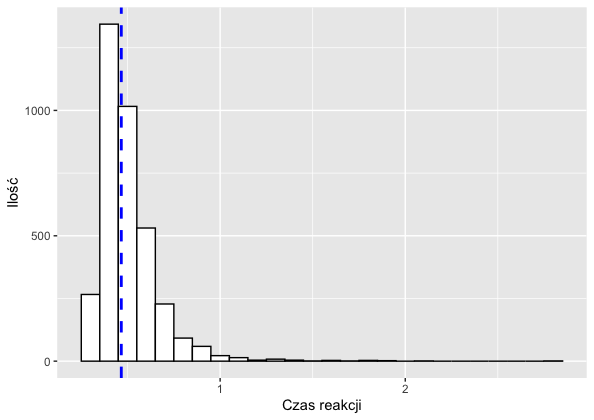
\includegraphics[scale=1]{hist1}
\label{Rysunek}
\end{figure}
\begin{center}
\section*{\large{\textbf{\textsc{Wyniki}}}}
\end{center}
Po sprawdzeniu normalności rozkładu i wybraniu typu testów statystycznych, zostały policzone podstawowe statystyki opisowe dla zbioru danych odbiegających od rozkładu normalnego - miary tendencji centralnej, zmienności oraz asymetrii. Były to mediana, rozstęp międzykwartylowy, odchylenie ćwiartkowe, pozycjny współczynnik zmienności oraz pozycyjny współczynnik asymetrii. Dla całego zbioru danych mediana ($Med$) wyniosła $0.47$, rozkład międzykwartylowy ($IQR$) wyniósł $0.16$, odchylenie ćwiartkowe ($Q_x$) przyjęło wartość $0.079$, współczynnik zmienności ($V_Q$) miał wartość $16.96$, zaś asymetria ($A_{Q_{x}}$) wyniosła $0.40$. Wyniki powyższych cech statystycznych dla 4 badanych grup zostały przedstawione w \textit{Tabeli 1}. Dodatkowo narysowano wykres \textit{box and whiskers plot} dla powyższych grup \textit{(Rysunek 2)}.
\begin{table}[h]
\caption{Statystyki opisowe}
\centering
\begin{tabular}{l c c c c c}
\hline\hline
Grupa & $Med$ & $IQR$ & $Q_x$ & $V_Q$ & $A_{Q_{x}}$ \\ [0.5ex]
\hline
Mandala i wysoka entropia&0.47&0.16&0.080&17.19&0.39 \\
Mandala i niska entropia&0.48&0.17&0.086&17.91&0.26 \\
Kartka i wysoka entropia&0.45&0.13&0.064&14.17&0.46 \\
Kartka i niska entropia&0.47&0.17&0.083&17.62&0.32 \\ [1ex]
\hline
\end{tabular}
\label{Tabela}
\end{table}
\begin{figure}[h]
\centering
\caption{Box and whiskers plot przedstawiający mediany wyników w grupach}
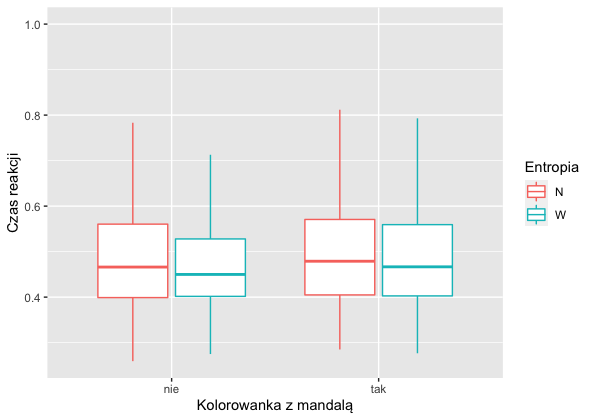
\includegraphics[scale=0.5]{box1}
\label{Rysunek}
\end{figure}
\paragraph{}
Poza opisem podstawowymi statystykami opisowymi przeprowadzono testy statystyczne badająće związek pomiędzy badanymi zmiennymi. Były to testy nieparametryczne. Były to testy badające osobne zależności między badanymi zmiennymi, oraz analiza wariancji dla wszystkich badanych zmiennych i ich interakcji. Wartości $p$ dla każdego z tych testów zostały przedstawione w \textit{Tabeli 2}.
\begin{table}[h]
\caption{Wartości $p$ obliczonych testów statystycznych}
\centering
\begin{tabular}{l c c c}
\hline\hline
 & Entropia & Kolorowanka & Interakcja \\ [0.5ex]
\hline
 & & Test U Manna-Whitneya& \\
 &$0.0045$&-&- \\
\hline
 & & Test Wilcoxona & \\
Czas reakcji&-&$0.017$&- \\ 
\hline
 & & Analiza wariancji & \\
 &$3.69*10^{-5}$&$0.27$&$0.015$ \\
\hline
\end{tabular}
\label{Tabela}
\end{table}
\paragraph{}
Jak wynika z powyższych danych, wszystkie zależności są istotne statystycznie na poziomie istotności $\alpha = 0.05$ poza zależnością między faktem kolorowania, a czasem reakcji uzyskanym w teście uwagi, obliczonej za pomocą analizy wariancji. Różnica ta może wynikać z nieparanetryczności rozkładum, jak również z tego, że zmienna kolorowania mandali przeprowadzona była w grupach zależnych.
\paragraph{}
Wartości siły efektu dla obu grup są nieistotne. Dla wpływu kolorowania na czas reakcji w teście uwagi wartość współczynnika d Cohena wyniosła $0.037$, zaś dla wpływu entropii otoczenia na czas reakcji w teście uwagi wzrokowej wartość współczynnika d Cohena wyniosła $0.20$.
\paragraph{}
Dodatkowo pomimo braku tej predykcji w pytaniu badawczym oraz w hipotezie, zauważono iż może istnieć związek pomiędzy typem bodźca wzrokowego, a czasem reakcji oraz, że w przypadku różnych entropii otoczenia wyniki się różnią. W tym celu przeprowadzono test Kruskala-Wallisa oraz analizę wariancji z których wynika, że istnieje istotnie statystyczny związek między typem bodźca, a czasem reakcji oraz, że istnieje istotna interakcja między typem bodźca, a entriopią otoczenia. Wartości $p$ tych badań przedstawiono w \textit{Tabeli 3}, zaś graficzne różnice zostały przedstawione na poniższym wykresie \textit{box and whiskers plot (Rysunek 3)}.
\begin{table}[h]
\caption{Wartości $p$ obliczonych testów statystycznych}
\centering
\begin{tabular}{l c c c}
\hline\hline
 & Typ & & Interakcja z entropią \\ [0.5ex]
\hline
 & &Test Kruskala-Wallisa & \\ [2ex]
Czas reakcji&$<2.2*10^{-16}$& &- \\
\hline
 & &Analiza wariancji& \\ [2ex]
Czas reakcji&$<2.2*10^{-16}$& &$0.011$ \\
\hline
\end{tabular}
\label{Tabela}
\end{table}
\begin{figure}[h]
\centering
\caption{Box and whiskers plot przedstawiający mediany wyników w grupach}
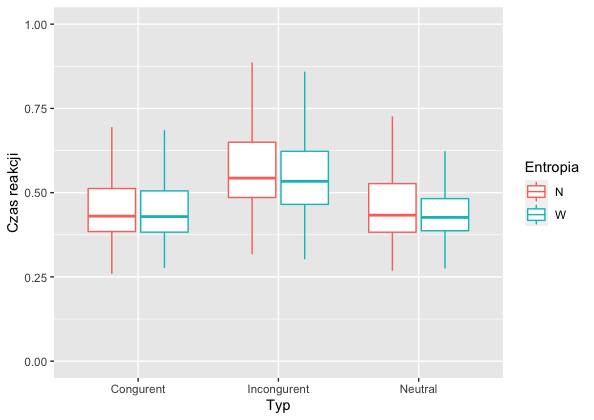
\includegraphics[scale=0.5]{box2}
\label{Rysunek}
\end{figure}
\begin{center}
\section*{\large{\textbf{\textsc{Dyskusja}}}}
\end{center}
\newpage
\bibliography{Biblio}
\end{document}